\chapter{工程问题二}
\section{例题分析}
\begin{example}
    一项工程,甲、乙两队合作需12 天完成,乙、丙两队合作需15 天完成,甲、
丙两队合作需20 天完成,如果由甲、乙、丙三队合作需几天完成?
\end{example}
\vspace{2cm}
\begin{example}
    加工一批零件,甲、乙合作24 天可以完成。现在由甲先做16 天,然后乙再
    做12 天,还剩下这批零件的$\frac{2}{5}$ 没有完成。已知甲每天比乙多加工3 个零件,求这
    批零件共多少个?
\end{example}
\vspace{2cm}
\begin{example}
    一项工程,甲单独完成需12 天,乙单独完成需9 天。若甲先做若干天后乙接
着做,共用10 天完成,问甲做了几天?
\end{example}
\vspace{2cm}
\begin{example}
    一件工作,甲、乙两人合作36 天完成,乙、丙两人合作45 天完成,甲、丙两人
合作要60 天完成。问甲一人独做需要多少天完成?
\end{example}
\vfill
\begin{example}
    做一批儿童玩具,甲组单独做10 天完成,乙组单独做12 天完成,丙组每天可生
产64 件。如果让甲、乙两组合作4 天,则还有256 件没完成。现在决定三个组合做
这批玩具,需要多少天完成?
\end{example}
\vfill
\begin{example}
    一项工程,甲、乙单独做分别需要18 天和27 天。如果甲做若干天后,乙接着
做,共用20 天完成。求甲、乙完成工作量之比。
\end{example}
\newpage
\vspace{2cm}
\begin{example}
    甲、乙两人共同加工一批零件, 8 小时可以完成任务。如果甲单独加工,便需要
12 小时完成。现在甲、乙两人共同生产了2$\frac{2}{5}$小时后,甲被调出做其他工作,由乙
继续生产了420 个零件才完成任务。问乙一共加工零件多少个?
\end{example}
\vspace{2cm}
\begin{example}
    有一个蓄水池,甲、乙两管同时打开, 9 分钟注满水池。现在,先打开甲管, 10
分钟后,再打开乙管, 3 分钟就注满水池。已知甲管比乙管每分钟多注入0.6 立方
米水,这个水池的容积是多少立方米?
\end{example}
\vspace{2cm}
\begin{example}
    修一段公路,甲队独做要用40 天,乙队独做要用24 天。现在两队同时从两端开
工,结果在距中点750 米处相遇。这段公路长多少米?
\end{example}
\vspace{2cm}
\begin{example}
    制作一批零件,甲车间要10 天完成,如果甲车间与乙车间一起做只要6 天就
能完成。乙车间与丙车间一起做,需要8 天才能完成。现在三个车间一起做,完成
后发现甲车间比乙车间多制作零件2400 个。问丙车间制作了多少个零件?
\end{example}
\vspace{4em}
\begin{example}
    一项工程,甲单独做要12 小时完成,乙单独做要18 小时完成.若甲先做1
小时,然后乙接替甲做1 小时,再由甲接替乙做1 小时,两人如此交替工作,问完
成任务时,共用了多少小时?
\end{example}
\begin{tikzpicture}
\draw[step=1cm,color=red!40] (-2cm,-2cm) grid (2cm,2cm);  
\draw[red] (0,0)--(2cm,2cm);
\draw[red,<->](-2cm,2cm)--(-2cm,0)--(2cm,0);
\draw (0,0) circle(1cm);
\draw [red] (0,0) ellipse (1cm and 0.5cm);
\draw [green] (0,0) arc (0:90:1cm); 
\draw [red,thick](-1cm,-1cm ) rectangle (1cm,1cm);
\node [below right]  at (0,0)  {n};
\node [red,below right] at (1cm,2cm) {你};

\end{tikzpicture}
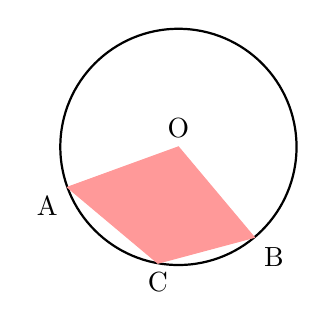
\begin{tikzpicture}
    \draw [thick](0,0) circle(1.5cm);
    \filldraw [red!40] (0,0)--(200:1.5cm)--(260:1.5cm)--(310:1.5cm)--cycle;
   \node [above] (0,0) {O};
   \node [below left] at (200:1.5cm) {A};
   \node [below] at (260:1.5cm) {C};
   \node [below right] at (310:1.5cm) {B};
\end{tikzpicture}
\begin{asy}
    size(200,0);
    draw((0,3)--(2,3),Arrow);
    draw((0,2)--(2,2),EndArrow);
    draw((0,1)--(2,1),BeginArrow);
    draw((0,0)--(2,0),Arrows);
    draw((0,-1)--(2,-1),MidArrow);
\end{asy}
